%package list
\documentclass{article}
\usepackage[top=3cm, bottom=3cm, outer=3cm, inner=3cm]{geometry}
\usepackage{multicol}
\usepackage{graphicx}
\usepackage{url}
%\usepackage{cite}
\usepackage{hyperref}
\usepackage{array}
%\usepackage{multicol}
\newcolumntype{x}[1]{>{\centering\arraybackslash\hspace{0pt}}p{#1}}
\usepackage{natbib}
\usepackage{pdfpages}
\usepackage{multirow}
\usepackage[normalem]{ulem}
\useunder{\uline}{\ul}{}
\usepackage{svg}
\usepackage{xcolor}
\usepackage{listings}
\lstdefinestyle{ascii-tree}{
	literate={├}{|}1 {─}{--}1 {└}{+}1 
}
\lstset{basicstyle=\ttfamily,
	showstringspaces=false,
	commentstyle=\color{red},
	keywordstyle=\color{blue}
}
%\usepackage{booktabs}
\usepackage{caption}
\usepackage{subcaption}
\usepackage{float}
\usepackage{array}

\newcolumntype{M}[1]{>{\centering\arraybackslash}m{#1}}
\newcolumntype{N}{@{}m{0pt}@{}}


%%%%%%%%%%%%%%%%%%%%%%%%%%%%%%%%%%%%%%%%%%%%%%%%%%%%%%%%%%%%%%%%%%%%%%%%%%%%
%%%%%%%%%%%%%%%%%%%%%%%%%%%%%%%%%%%%%%%%%%%%%%%%%%%%%%%%%%%%%%%%%%%%%%%%%%%%
\newcommand{\itemEmail}{jchuraaca@unsa.edu.pe}
\newcommand{\itemStudent}{Julio Rubén Chura Acabana}
\newcommand{\itemCourse}{ F. de Programción 2}
\newcommand{\itemCourseCode}{20230472}
\newcommand{\itemSemester}{I}
\newcommand{\itemUniversity}{Universidad Nacional de San Agustín de Arequipa}
\newcommand{\itemFaculty}{Facultad de Ingeniería de Producción y Servicios}
\newcommand{\itemDepartment}{Departamento Académico de Ingeniería de Sistemas e Informática}
\newcommand{\itemSchool}{Escuela Profesional de Ingeniería de Sistemas}
\newcommand{\itemAcademic}{2023 - B}
\newcommand{\itemInput}{Del 11 de Octubre 2023}
\newcommand{\itemOutput}{Al 16 de octubre 2023}
\newcommand{\itemPracticeNumber}{05}
\newcommand{\itemTheme}{Arreglos Bidimensionales de Objetos}
%%%%%%%%%%%%%%%%%%%%%%%%%%%%%%%%%%%%%%%%%%%%%%%%%%%%%%%%%%%%%%%%%%%%%%%%%%%%
%%%%%%%%%%%%%%%%%%%%%%%%%%%%%%%%%%%%%%%%%%%%%%%%%%%%%%%%%%%%%%%%%%%%%%%%%%%%

\usepackage[english,spanish]{babel}
\usepackage[utf8]{inputenc}
\AtBeginDocument{\selectlanguage{spanish}}
\renewcommand{\figurename}{Figura}
\renewcommand{\refname}{Referencias}
\renewcommand{\tablename}{Tabla} %esto no funciona cuando se usa babel
\AtBeginDocument{%
	\renewcommand\tablename{Tabla}
}

\usepackage{fancyhdr}
\pagestyle{fancy}
\fancyhf{}
\setlength{\headheight}{30pt}
\renewcommand{\headrulewidth}{1pt}
\renewcommand{\footrulewidth}{1pt}
\fancyhead[L]{\raisebox{-0.2\height}{
\includegraphics[width=3cm]{img/logo_episunsa.png}}}
\fancyhead[C]{\fontsize{7}{7}\selectfont	\itemUniversity \\ \itemFaculty \\ \itemDepartment \\ \itemSchool \\ \textbf{\itemCourse}}
\fancyhead[R]{\raisebox{-0.2\height}{
\includegraphics[width=1.2cm]{img/logo_abet}}}
\fancyfoot[L]{Estudiante Julio Rubén Chura Acabana}
\fancyfoot[C]{\itemCourse}
\fancyfoot[R]{Página \thepage}

% para el codigo fuente
\usepackage{listings}
\usepackage{color, colortbl}
\definecolor{dkgreen}{rgb}{0,0.6,0}
\definecolor{gray}{rgb}{0.5,0.5,0.5}
\definecolor{mauve}{rgb}{0.58,0,0.82}
\definecolor{codebackground}{rgb}{0.95, 0.95, 0.92}
\definecolor{tablebackground}{rgb}{0.8, 0, 0}

\lstset{frame=tb,
	language=bash,
	aboveskip=3mm,
	belowskip=3mm,
	showstringspaces=false,
	columns=flexible,
	basicstyle={\small\ttfamily},
	numbers=none,
	numberstyle=\tiny\color{gray},
	keywordstyle=\color{blue},
	commentstyle=\color{dkgreen},
	stringstyle=\color{mauve},
	breaklines=true,
	breakatwhitespace=true,
	tabsize=3,
	backgroundcolor= \color{codebackground},
}

\begin{document}
	
	\vspace*{10px}
	
	\begin{center}	
		\fontsize{17}{17} \textbf{ Informe de Laboratorio \itemPracticeNumber}
	\end{center}
	\centerline{\textbf{\Large Tema: \itemTheme}}
	%\vspace*{0.5cm}	
	
	\begin{flushright}
		\begin{tabular}{|M{2.5cm}|N|}
			\hline 
			\rowcolor{tablebackground}
			\color{white} \textbf{Nota}  \\
			\hline 
			\\[30pt]
			\hline 			
		\end{tabular}
	\end{flushright}	
	
	\begin{table}[H]
		\begin{tabular}{|x{4.7cm}|x{4.8cm}|x{4.8cm}|}
			\hline 
			\rowcolor{tablebackground}
			\color{white} \textbf{Estudiante} & \color{white}\textbf{Escuela}  & \color{white}\textbf{Asignatura}   \\
			\hline 
			{\itemStudent \par \itemEmail} & \itemSchool & {\itemCourse \par Semestre: \itemSemester \par Código: \itemCourseCode}     \\
			\hline 			
		\end{tabular}
	\end{table}		
	
	\begin{table}[H]
		\begin{tabular}{|x{4.7cm}|x{4.8cm}|x{4.8cm}|}
			\hline 
			\rowcolor{tablebackground}
			\color{white}\textbf{Laboratorio} & \color{white}\textbf{Tema}  & \color{white}\textbf{Duración}   \\
			\hline 
			\itemPracticeNumber & \itemTheme & 04 horas   \\
			\hline 
		\end{tabular}
	\end{table}
	
	\begin{table}[H]
		\begin{tabular}{|x{4.7cm}|x{4.8cm}|x{4.8cm}|}
			\hline 
			\rowcolor{tablebackground}
			\color{white}\textbf{Semestre académico} & \color{white}\textbf{Fecha de inicio}  & \color{white}\textbf{Fecha de entrega}   \\
			\hline 
			\itemAcademic & \itemInput &  \itemOutput  \\
			\hline 
		\end{tabular}
	\end{table}
	
	\section{Tarea}
	\begin{itemize}		
		\item 
		Inicializar el tablero con n soldados aleatorios entre 1 y 10. Cada soldado tendrá un nombre 
		autogenerado: Soldado0, Soldado1, etc., un valor de puntos de vida autogenerado 
		aleatoriamente [1..5], la fila y columna también autogenerados aleatoriamente (no puede 
		haber 2 soldados en el mismo cuadrado). Se debe mostrar el tablero con todos los soldados creados. Además de los datos del Soldado con mayor vida, 
		el promedio de puntos de vida de todos los soldados creados, el nivel de vida de todo el ejército, los datos de todos los soldados en el orden que fueron creados y un ranking de poder de todos los soldados creados, del que tiene más nivel de vida al que tiene menos (usar al 
		menos 2 algoritmos de ordenamiento)
		
		\item Usted debe realizar varios commits y al término de la actividad deberá realizar un informe
		
	\end{itemize}
	
	\section{Equipos, materiales y temas utilizados}
	\begin{itemize}
		\item Sistema Operativo Windows
		\item Notepad++ v8.5.4
		\item OpenJDK 64-Bits 20.0.2.
		\item Git 2.42.0.
		\item Cuenta en GitHub con el correo institucional.
		\item Arreglos Bidimensionales de objetos
	\end{itemize}
	
	\section{URL de Repositorio Github}
	\begin{itemize}
		\item URL del Repositorio GitHub para clonar o recuperar.
		\item \url{https://github.com/JulioChura/fp2-23b.git}
		\item URL para el laboratorio 01 en el Repositorio GitHub.
		\item \url{https://github.com/JulioChura/fp2-23b/tree/main/fase01/lab05}
	\end{itemize}
	
	\section{Actividades con el repositorio GitHub}
	
	
	\begin{lstlisting}[language=bash,caption={Se iniciliaza el espacio de trabajo y se modifca la clase Soldier.java}][H]
		mkdir lab05
		cd lab03
		Copy-Item "Soldier.java" -Destination "..\lab05"
		Copy-Item "VideoJuego.java" -Destination "..\lab05"
		cd ..
		cd lab05
		notepad++ Soldier.java
	\end{lstlisting}
	
	\begin{figure}[H]
		\centering
		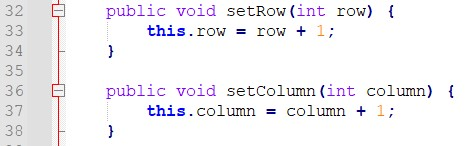
\includegraphics[width=0.7\textwidth,keepaspectratio]{img/1.jpg}
		%\includesvg{img/automata.svg}
		%\label{img:mot2}
		%\caption{Product backlog.}
	\end{figure}
		
	
	\begin{itemize}	
		\item Se han borrado líneas de código del lab03 para poder realizar la actividad lab05 
		\item En la clase Soldier.java se aumentan los atributos row y column junto con sus Getters y Setters. En los Setters de row y column se le suma uno ya que el usuario está acostumbrado a que se empiece a contar desde la posición uno y no desde la cero como lo hace el lenguaje de programación.
	\end{itemize}
	

	
	\begin{lstlisting}[language=bash,caption={Commit: "Se ha adaptado VideoJuego.java del lab03 para el lab05, pero no se ha avanzado nada" }][H]
		git add VideoJuego.java
		git commit -m  git commit -m "Se ha adaptado VideoJuego.java del lab03 para el lab05 pero no se ha avanzado nada"
		git push -u origin main
		git add Soldier.java
		git add Soldier.java
	   git commit -m  git commit -m "La clase Soldier.java esta termida"
	   git push -u origin main
	\end{lstlisting}
	
	
	
	
	
		
	\begin{lstlisting}[language=bash,caption={ Se crea un método para generar el arreglo bidimensional de tipo Soldier }][H]
	notepad++ VideoJuego.java	
	\end{lstlisting}
	
	\begin{figure}[H]
		\centering
		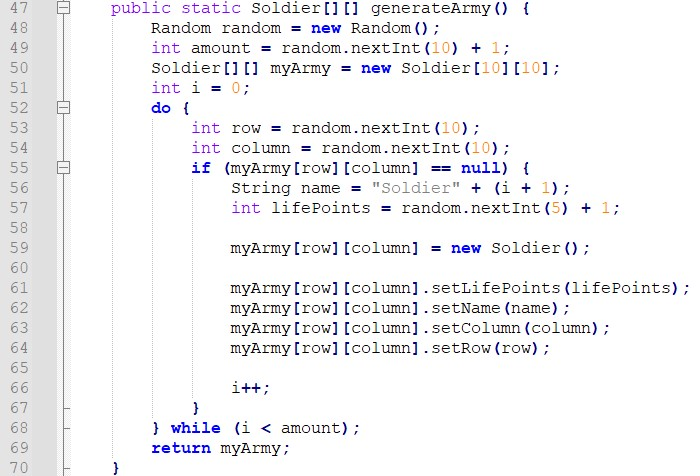
\includegraphics[width=0.8\textwidth,keepaspectratio]{img/2.jpg}
		%\includesvg{img/automata.svg}
		%\label{img:mot2}
		%\caption{Product backlog.}
	\end{figure}
	
	\begin{itemize}	
		\item En el método generateArmy() se crea un arreglo bidimensional de 10 filas y 10 columnas con el fin de cubrir la misma cantidad de casillas del tablero según la práctica del laboratorio, por lo que habrán posiciones que quedarán vacías ya que la cantidad de elementos del arreglo será una cantidad aleatoria que oscila entre 1 a 10. También se genera el nombre de cada Soldier y sus puntos de vida de forma aleatoria. Este arreglo nos servirá más que nada para imprimir el tablero de una forma más sencilla
	\end{itemize}	
		
	\begin{lstlisting}[language=bash,caption={Commit: Se ha creado el metodo que permite generar un arreglo de soldados sin repetir posiciones }][H]
		git VideoJuego.java
		git commit -m  git commit -m "Se ha creado el metodo que permite generar un arreglo de soldados sin repetir posiciones"
		git push -u origin main
	\end{lstlisting}
	
	
	
	\begin{lstlisting}[language=bash,caption={ Se crea un metodo que genera un arreglo unidimensional  }][H]
		notepad++ VideoJuego.java	
	\end{lstlisting}
	
		
	\begin{figure}[H]
		\centering
		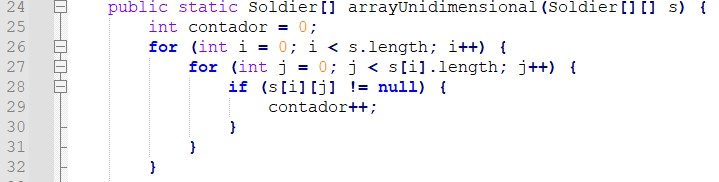
\includegraphics[width=0.8\textwidth,keepaspectratio]{img/3.jpg}
		%\includesvg{img/automata.svg}
		%\label{img:mot2}
		%\caption{Product backlog.}
	\end{figure}	
		
		
	\begin{itemize}	
		\item Este método se crea con el propósito de generar un arreglo unidimensional a partir del arreglo bidimensional ya creado, ya que nos facilitará el trabajo con los demás métodos que la práctica de laboratorio requiere. De hecho, antes de crear este método, había otro que podía imprimir los elementos del arreglo bidimensional, pero fue reemplazado porque era necesario. Además, el método imprimir ya contenía líneas de código que permitían la creación del arreglo unidimensional, por lo que habría repetición de código
	\end{itemize}		
		
		
		
	\begin{lstlisting}[language=bash,caption={Commit:  Se reemplaza el metodo de imprimir por el de generar arreglo unidimensional para poder trabajar los demas metodos }][H]
		git add VideoJuego.java
		git commit -m  git commit -m " Se reemplaza el metodo de imprimir por el de generar arreglo unidimensional para poder trabajar los demas metodos"
		git push -u origin main
	\end{lstlisting}
		
		
		
		
	\begin{lstlisting}[language=bash,caption={ Método para imprimir el tablero con la posición de cada soldado }][H]
		notepad++ VideoJuego.java
	\end{lstlisting}
		
	\begin{figure}[H]
		\centering
		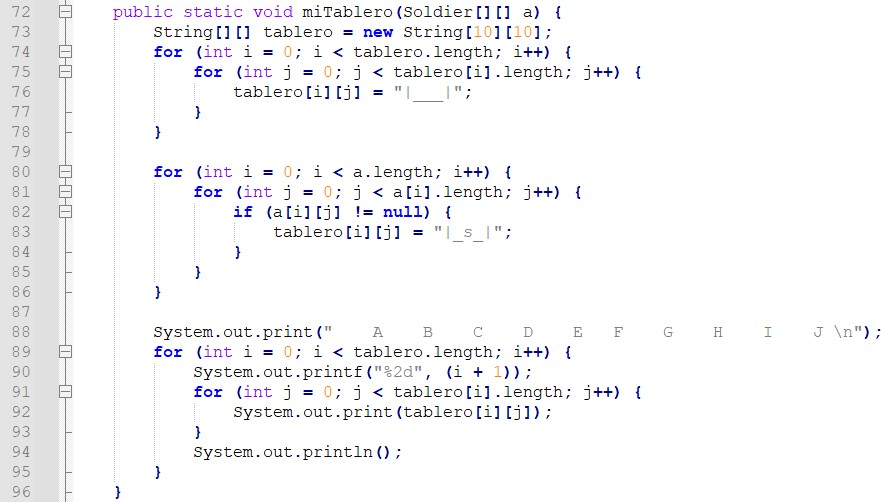
\includegraphics[width=1\textwidth,keepaspectratio]{img/4.jpg}
		%\includesvg{img/automata.svg}
		%\label{img:mot2}
		%\caption{Product backlog.}
	\end{figure}	
		
	\begin{itemize}	
			\item Esta es la versión final del método. Las primeras versiones generaban un tablero bidimensional y en el main se hacía el reemplazo de los carácteres a "s", como también las entradas del tablero, sin embargo, para que haya un orden, se decide que en el metodo miTablero ya se pueda mostrar el tablero con los soldados ubicados en él y las entradas que están en el borde del tablero
			\item En el main se escribe la línea de código que hace llamado al método
	\end{itemize}
	
	\begin{lstlisting}[language=bash,caption={ Probando el tablero  }][H]
		javac VideoJuego.java
		java VideoJuego
		    A    B      C    D    E      F    G    H    I    J
		1 |___||___||___||_s_||___||___||___||___||___||___|
		2 |___||___||___||___||___||___||___||___||_s_||___|
		3 |_s_||___||___||___||___||___||___||___||___||___|
		4 |___||___||___||___||___||___||___||___||___||___|
		5 |___||___||___||___||___||___||___||___||___||___|
		6 |___||_s_||___||_s_||___||___||___||___||___||___|
		7 |___||___||___||___||___||___||___||___||___||___|
		8 |_s_||___||___||___||___||___||___||___||___||___|
		9 |___||_s_||___||___||___||___||___||___||___||___|
		10|_s_||___||___||___||___||___||___||___||___||___|
		
	\end{lstlisting}
	
	
	\begin{lstlisting}[language=bash,caption={Commit:  Se ha organizado la forma en la que se muestra el tablero, ahora está en un método }][H]
		git add VideoJuego.java
		git commit -m  git commit -m "Se ha organizado la forma en la que se muestra el tablero, ahora esta en un metodo"
		git push -u origin main
	\end{lstlisting}	
		
		
	\begin{lstlisting}[language=bash,caption={Método de ordenamiento por inserción y también la impresión de los datos de acuerdo a su orden de creación}][H]
		notepad++ VideoJuego.java
	\end{lstlisting}	
		
	

	\begin{figure}[H]
		\centering
		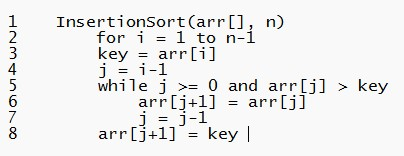
\includegraphics[width=0.7\textwidth,keepaspectratio]{img/insertion.jpg}
		%\includesvg{img/automata.svg}
		%\label{img:mot2}
		%\caption{Product backlog.}
	\end{figure}	
	
	\begin{itemize}	
		\item Este vendría a ser el pseudocódigo del método de ordenamiento por inserción
	\end{itemize}
		
		
	\begin{figure}[H]
		\centering
		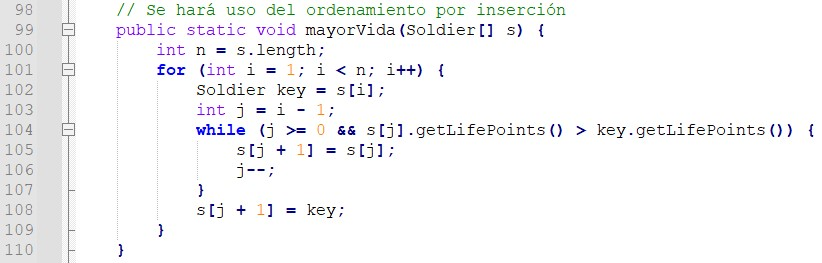
\includegraphics[width=1.2\textwidth,keepaspectratio]{img/5.jpg}
		%\includesvg{img/automata.svg}
		%\label{img:mot2}
		%\caption{Product backlog.}
	\end{figure}	
		
	\begin{itemize}	
		\item Este vendría a ser el algoritmo de ordenamiento por inserción, pero adaptado a las necesidades del problema. Se implementa este algoritmo para que pueda ordenar el arreglo de menor a mayor ya que en una de las pautas del problema se nos exige usar dos algoritmos de ordenamiento,este vendría a ser el primero. En el main se escribe código el cual mostrará el último elemento del arreglo
	\end{itemize}
		
	\begin{figure}[H]
		\centering
		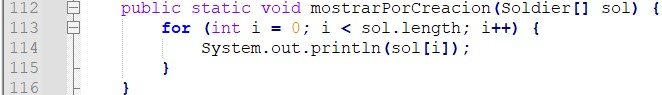
\includegraphics[width=0.8\textwidth,keepaspectratio]{img/6.jpg}
		%\includesvg{img/automata.svg}
		%\label{img:mot2}
		%\caption{Product backlog.}
	\end{figure}
	 
	
	\begin{itemize}	
		\item Como ya se mencionó, el método de mostrar los datos del arreglo Soldier ya estaba culminado, sin embargo por razones ya explicadas se decide cambiarlo e implementarlo después. En esta versión se opta por imprimir los datos de un arreglo unidimensional 
	\end{itemize}
		
	\begin{figure}[H]
		\centering
		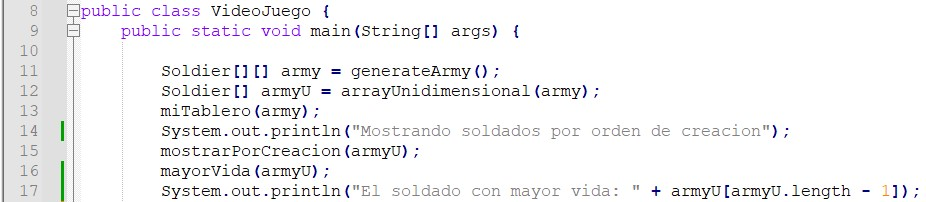
\includegraphics[width=1.2\textwidth,keepaspectratio]{img/7.jpg}
		%\includesvg{img/automata.svg}
		%\label{img:mot2}
		%\caption{Product backlog.}
	\end{figure}
		
	\begin{itemize}	
		\item En el main están las líneas de código que permitirán mostrar como funcionan estos dós métodos
	\end{itemize}	
		
	\begin{lstlisting}[language=bash,caption={ Compilación de los métodos creados hasta el momento }][H]
		javac VideoJuego.java
		java VideoJuego
		    A    B    C      D     E     F    G    H     I    J
		1 |___||___||___||___||___||___||___||___||_s_||___|
		2 |___||___||___||___||___||___||___||___||_s_||___|
		3 |___||___||___||___||___||___||_s_||___||___||___|
		4 |___||___||___||___||___||___||___||___||___||___|
		5 |___||_s_||___||___||___||___||___||___||___||___|
		6 |___||___||___||___||___||___||___||___||___||___|
		7 |___||___||___||___||___||___||___||___||___||___|
		8 |_s_||___||_s_||___||___||___||___||___||___||___|
		9 |___||_s_||___||___||___||___||___||___||___||___|
		10|___||___||___||___||___||___||___||___||___||_s_|
		Mostrando soldados por orden de creacion
		Soldier [name=Soldier7, lifePoints=5, row=1, column=9]
		Soldier [name=Soldier5, lifePoints=2, row=2, column=9]
		Soldier [name=Soldier3, lifePoints=5, row=3, column=7]
		Soldier [name=Soldier2, lifePoints=4, row=5, column=2]
		Soldier [name=Soldier8, lifePoints=3, row=8, column=1]
		Soldier [name=Soldier6, lifePoints=5, row=8, column=3]
		Soldier [name=Soldier4, lifePoints=1, row=9, column=2]
		Soldier [name=Soldier1, lifePoints=4, row=10, column=10]
		El soldado con mayor vida: Soldier [name=Soldier6, lifePoints=5, row=8, column=3]	
	\end{lstlisting}
		
		
		
	\begin{lstlisting}[language=bash,caption={ Se crea el método que calcula el promedio y puntos de vida total del ejército }][H]
		notepad++ VideoJuego.java	
	\end{lstlisting}	
		
		
	\begin{figure}[H]
		\centering
		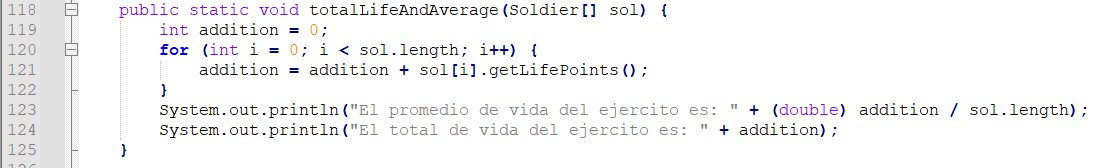
\includegraphics[width=1.09\textwidth,keepaspectratio]{img/8.jpg}
		%\includesvg{img/automata.svg}
		%\label{img:mot2}
		%\caption{Product backlog.}
	\end{figure}	
		
	\begin{itemize}	
		\item Debido a que el promedio de vida del ejército se calcula en base a la suma de este, se decide que ambos valores se calculen en un mismo método y se impriman desde ya en el mismo método. De la misma manera que se hizo con los demás métodos, en el main se escribe una línea de código que llama a este método 
	\end{itemize}	
		
	\begin{lstlisting}[language=bash,caption={ Compilando y probando el método totaLifeAndAverage y demás}][H]
		javac VideoJuego.java
		java VideoJuego
		    A    B    C    D    E   F    G    H    I    J
		1 |___||___||___||___||___||___||___||_s_||___||___|
		2 |___||___||___||_s_||___||___||___||___||___||___|
		3 |___||_s_||___||___||___||___||___||___||___||___|
		4 |_s_||___||___||___||___||___||___||___||___||___|
		5 |___||___||___||___||___||___||___||___||___||___|
		6 |___||___||___||___||___||___||___||___||___||___|
		7 |___||___||___||___||___||___||___||___||___||___|
		8 |___||___||___||___||___||___||___||___||___||___|
		9 |___||___||___||___||_s_||___||_s_||___||___||___|
		10|___||_s_||___||___||___||___||___||___||___||___|
		Mostrando soldados por orden de creacion
		Soldier [name=Soldier7, lifePoints=5, row=1, column=8]
		Soldier [name=Soldier2, lifePoints=2, row=2, column=4]
		Soldier [name=Soldier1, lifePoints=5, row=3, column=2]
		Soldier [name=Soldier3, lifePoints=5, row=4, column=1]
		Soldier [name=Soldier5, lifePoints=4, row=9, column=5]
		Soldier [name=Soldier6, lifePoints=2, row=9, column=7]
		Soldier [name=Soldier4, lifePoints=3, row=10, column=2]
		El soldado con mayor vida: Soldier [name=Soldier3, lifePoints=5, row=4, column=1]
		El promedio de vida del ejercito es: 3.7142857142857144
		El total de vida del ejercito es: 26	
	\end{lstlisting}
		
		
	\begin{lstlisting}[language=bash,caption={Commit: "Se ha creado el metodo que calcula el promedio y total de los puntos de vida" }][H]
		git add VideoJuego.java
		git commit -m  git commit -m "Se ha creado el metodo que calcula el promedio y total de los puntos de vida"
		git push -u origin main
	\end{lstlisting}
		
		
	
		
		
	
		
	
	\begin{lstlisting}[language=bash,caption={ Método burbuja que muestra el ranking de poder (vida) }][H]
		notepad++ VideoJuego.java	
	\end{lstlisting}
	
	
	\begin{figure}[H]
		\centering
		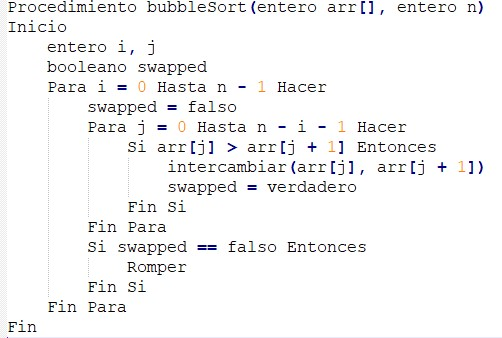
\includegraphics[width=0.8\textwidth,keepaspectratio]{img/burbuja.jpg}
		%\includesvg{img/automata.svg}
		%\label{img:mot2}
		%\caption{Product backlog.}
	\end{figure}

	
	\begin{itemize}	
		\item Este el pseudocódigo del ordenamiento burbuja 
	\end{itemize}
	
	\begin{figure}[H]
		\centering
		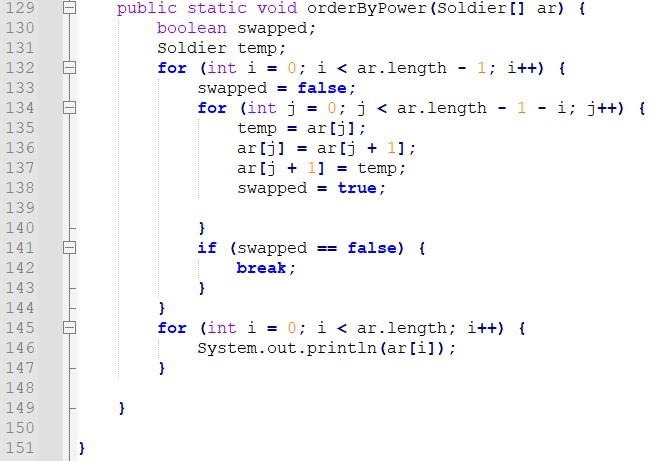
\includegraphics[width=0.9\textwidth,keepaspectratio]{img/9.jpg}
		%\includesvg{img/automata.svg}
		%\label{img:mot2}
		%\caption{Product backlog.}
	\end{figure}
	
	\begin{itemize}	
		\item Este es el método burbuja ya implementado a las necesidades del código. En el método se decide incluir la impresión de los elementos ordenados ya que el método debe mostrar un ranking de acuerdo a la vida
	\end{itemize}
	
	
	\begin{lstlisting}[language=bash,caption={ Compilando y probando todos los métodos solicitados en la práctica }][H]
		     A    B    C     D    E     F     G    H     I    J
		1 |___||___||___||___||___||_s_||___||___||___||___|
		2 |___||___||___||___||___||___||___||___||___||___|
		3 |___||___||___||_s_||___||___||___||___||___||___|
		4 |___||___||___||___||___||___||___||___||___||___|
		5 |___||___||___||_s_||___||___||___||___||___||___|
		6 |___||___||___||___||___||___||___||___||___||___|
		7 |_s_||___||___||___||___||___||___||___||___||___|
		8 |___||___||___||___||___||___||___||___||___||___|
		9 |___||___||___||___||___||___||___||___||___||___|
		10|___||___||___||___||_s_||___||___||___||___||_s_|
		Mostrando soldados por orden de creacion
		Soldier [name=Soldier3, lifePoints=3, row=1, column=6]
		Soldier [name=Soldier6, lifePoints=3, row=3, column=4]
		Soldier [name=Soldier5, lifePoints=1, row=5, column=4]
		Soldier [name=Soldier4, lifePoints=1, row=7, column=1]
		Soldier [name=Soldier1, lifePoints=3, row=10, column=5]
		Soldier [name=Soldier2, lifePoints=4, row=10, column=10]
		El soldado con mayor vida: Soldier [name=Soldier2, lifePoints=4, row=10, column=10]
		El promedio de vida del ejercito es: 2.5
		El total de vida del ejercito es: 15
		Mostrando soldados por ranking de poder
		Soldier [name=Soldier2, lifePoints=4, row=10, column=10]
		Soldier [name=Soldier1, lifePoints=3, row=10, column=5]
		Soldier [name=Soldier6, lifePoints=3, row=3, column=4]
		Soldier [name=Soldier3, lifePoints=3, row=1, column=6]
		Soldier [name=Soldier4, lifePoints=1, row=7, column=1]
		Soldier [name=Soldier5, lifePoints=1, row=5, column=4]
		
	\end{lstlisting}
	
	
	
	\begin{lstlisting}[language=bash,caption={ Commit: Metodo burbuja que muestra el ranking de poder }][H]
		git add VideoJuego.java
		git commit -m  git commit -m "Metodo burbuja que muestra el ranking de poder"
		git push -u origin main
	\end{lstlisting}
	
	
	\begin{lstlisting}[language=bash,caption={ Estructura del main }][H]
		notepad++ VideoJuego.java	
	\end{lstlisting}
	\begin{figure}[H]
		\centering
		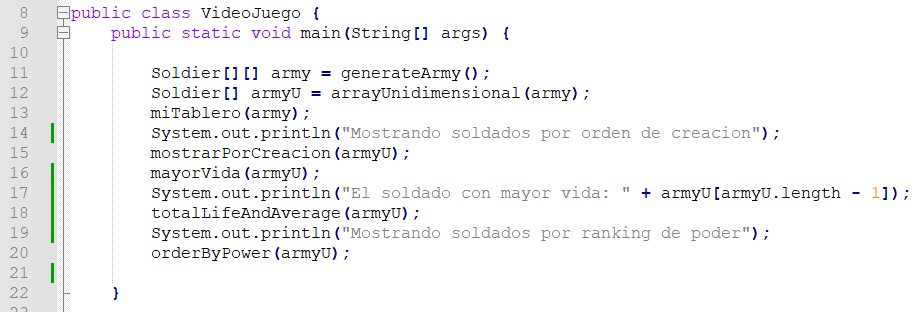
\includegraphics[width=1.1\textwidth,keepaspectratio]{img/10.jpg}
		%\includesvg{img/automata.svg}
		%\label{img:mot2}
		%\caption{Product backlog.}
	\end{figure}
	
	
	\subsection{Estructura de laboratorio 05}
	\begin{itemize}	
		\item El contenido que se entrega en este laboratorio es el siguiente:
	\end{itemize}
	
	\begin{lstlisting}[style=ascii-tree]
		
	lab05	
	|  Soldier.java
	|   VideoJuego.java
	
	└───latex
	|   |   programacion_lab05_rescobedoq_v1.0.pdf
	|   |   programacion_lab05_rescobedoq_v1.0.tex
	|   |
	|   └───img
	|       |   1.jpg
	|       |   10.jpg
	|       |   2.jpg
	|       |   3.jpg
	|       |   4.jpg
	|       |   5.jpg
	|       |   6.jpg
	|       |   7.jpg
	|       |   8.jpg
	|       |   9.jpg
	|       |   burbuja.jpg
	|       |   insertion.jpg
	|       |   logo_abet.png
	|       |   logo_episunsa.png
	|       |   logo_unsa.jpg            
	|
	└───src

	\end{lstlisting}    
	
	\section{\textcolor{red}{Rúbricas}}
	
	\subsection{\textcolor{red}{Entregable Informe}}
	\begin{table}[H]
		\caption{Tipo de Informe}
		\setlength{\tabcolsep}{0.5em} % for the horizontal padding
		{\renewcommand{\arraystretch}{1.5}% for the vertical padding
			\begin{tabular}{|p{3cm}|p{12cm}|}
				\hline
				\multicolumn{2}{|c|}{\textbf{\textcolor{red}{Informe}}}  \\
				\hline 
				\textbf{\textcolor{red}{Latex}} & \textcolor{blue}{El informe está en formato PDF desde Latex,  con un formato limpio (buena presentación) y facil de leer.}   \\ 
				\hline 
				
				
			\end{tabular}
		}
	\end{table}
	
	\clearpage
	
	\subsection{\textcolor{red}{Rúbrica para el contenido del Informe y demostración}}
	\begin{itemize}			
		\item El alumno debe marcar o dejar en blanco en celdas de la columna \textbf{Checklist} si cumplio con el ítem correspondiente.
		\item Si un alumno supera la fecha de entrega,  su calificación será sobre la nota mínima aprobada, siempre y cuando cumpla con todos lo items.
		\item El alumno debe autocalificarse en la columna \textbf{Estudiante} de acuerdo a la siguiente tabla:
		
		\begin{table}[ht]
			\caption{Niveles de desempeño}
			\begin{center}
				\begin{tabular}{ccccc}
					\hline
					& \multicolumn{4}{c}{Nivel}\\
					\cline{1-5}
					\textbf{Puntos} & Insatisfactorio 25\%& En Proceso 50\% & Satisfactorio 75\% & Sobresaliente 100\%\\
					\textbf{2.0}&0.5&1.0&1.5&2.0\\
					\textbf{4.0}&1.0&2.0&3.0&4.0\\
					\hline
				\end{tabular}
			\end{center}
		\end{table}	
		
	\end{itemize}
	
	\begin{table}[H]
		\caption{Rúbrica para contenido del Informe y demostración}
		\setlength{\tabcolsep}{0.5em} % for the horizontal padding
		{\renewcommand{\arraystretch}{1.5}% for the vertical padding
			%\begin{center}
			\begin{tabular}{|p{2.7cm}|p{7cm}|x{1.3cm}|p{1.2cm}|p{1.5cm}|p{1.1cm}|}
				\hline
				\multicolumn{2}{|c|}{Contenido y demostración} & Puntos & Checklist & Estudiante & Profesor\\
				\hline
				\textbf{1. GitHub} & Hay enlace URL activo del directorio para el  laboratorio hacia su repositorio GitHub con código fuente terminado y fácil de revisar. &2 &X &2 & \\ 
				\hline
				\textbf{2. Commits} &  Hay capturas de pantalla de los commits más importantes con sus explicaciones detalladas. (El profesor puede preguntar para refrendar calificación). &4 &X &3 & \\ 
				\hline 
				\textbf{3. Código fuente} &  Hay porciones de código fuente importantes con numeración y explicaciones detalladas de sus funciones. &2 &X &2 & \\ 
				\hline 
				\textbf{4. Ejecución} & Se incluyen ejecuciones/pruebas del código fuente  explicadas gradualmente. &2 &X &1 & \\ 
				\hline			
				\textbf{5. Pregunta} & Se responde con completitud a la pregunta formulada en la tarea.  (El profesor puede preguntar para refrendar calificación).  &2 &X &2 & \\ 
				\hline	
				\textbf{6. Fechas} & Las fechas de modificación del código fuente estan dentro de los plazos de fecha de entrega establecidos. &2 &X &2 & \\ 
				\hline 
				\textbf{7. Ortografía} & El documento no muestra errores ortográficos. &2 &X &2 & \\ 
				\hline 
				\textbf{8. Madurez} & El Informe muestra de manera general una evolución de la madurez del código fuente,  explicaciones puntuales pero precisas y un acabado impecable.   (El profesor puede preguntar para refrendar calificación).  &4 &X &3 & \\ 
				\hline
				\multicolumn{2}{|c|}{\textbf{Total}} &20 & &17 & \\ 
				\hline
			\end{tabular}
			%\end{center}
			%\label{tab:multicol}
		}
	\end{table}
	
	\clearpage
	
	\section{Referencias}
	\begin{itemize}			
		\item \url{https://www.geeksforgeeks.org/bubble-sort/}
		\item \url{https://www.geeksforgeeks.org/insertion-sort/}
		\item \url{https://drive.google.com/file/d/18wvjXuguiRaIZ3ZOdElzC-LM9hrabhue/view?usp=drive_link}
		
	\end{itemize}	
	
	%\clearpage
	%\bibliographystyle{apalike}
	%\bibliographystyle{IEEEtranN}
	%\bibliography{bibliography}
	
\end{document}